% Options for packages loaded elsewhere
% Options for packages loaded elsewhere
\PassOptionsToPackage{unicode}{hyperref}
\PassOptionsToPackage{hyphens}{url}
\PassOptionsToPackage{dvipsnames,svgnames,x11names}{xcolor}
%
\documentclass[
  spanish,
  letterpaper,
  DIV=11,
  numbers=noendperiod,
  oneside]{scrreprt}
\usepackage{xcolor}
\usepackage[left=1in,marginparwidth=2.0666666666667in,textwidth=4.1333333333333in,marginparsep=0.3in]{geometry}
\usepackage{amsmath,amssymb}
\setcounter{secnumdepth}{5}
\usepackage{iftex}
\ifPDFTeX
  \usepackage[T1]{fontenc}
  \usepackage[utf8]{inputenc}
  \usepackage{textcomp} % provide euro and other symbols
\else % if luatex or xetex
  \usepackage{unicode-math} % this also loads fontspec
  \defaultfontfeatures{Scale=MatchLowercase}
  \defaultfontfeatures[\rmfamily]{Ligatures=TeX,Scale=1}
\fi
\usepackage{lmodern}
\ifPDFTeX\else
  % xetex/luatex font selection
\fi
% Use upquote if available, for straight quotes in verbatim environments
\IfFileExists{upquote.sty}{\usepackage{upquote}}{}
\IfFileExists{microtype.sty}{% use microtype if available
  \usepackage[]{microtype}
  \UseMicrotypeSet[protrusion]{basicmath} % disable protrusion for tt fonts
}{}
\makeatletter
\@ifundefined{KOMAClassName}{% if non-KOMA class
  \IfFileExists{parskip.sty}{%
    \usepackage{parskip}
  }{% else
    \setlength{\parindent}{0pt}
    \setlength{\parskip}{6pt plus 2pt minus 1pt}}
}{% if KOMA class
  \KOMAoptions{parskip=half}}
\makeatother
% Make \paragraph and \subparagraph free-standing
\makeatletter
\ifx\paragraph\undefined\else
  \let\oldparagraph\paragraph
  \renewcommand{\paragraph}{
    \@ifstar
      \xxxParagraphStar
      \xxxParagraphNoStar
  }
  \newcommand{\xxxParagraphStar}[1]{\oldparagraph*{#1}\mbox{}}
  \newcommand{\xxxParagraphNoStar}[1]{\oldparagraph{#1}\mbox{}}
\fi
\ifx\subparagraph\undefined\else
  \let\oldsubparagraph\subparagraph
  \renewcommand{\subparagraph}{
    \@ifstar
      \xxxSubParagraphStar
      \xxxSubParagraphNoStar
  }
  \newcommand{\xxxSubParagraphStar}[1]{\oldsubparagraph*{#1}\mbox{}}
  \newcommand{\xxxSubParagraphNoStar}[1]{\oldsubparagraph{#1}\mbox{}}
\fi
\makeatother

\usepackage{color}
\usepackage{fancyvrb}
\newcommand{\VerbBar}{|}
\newcommand{\VERB}{\Verb[commandchars=\\\{\}]}
\DefineVerbatimEnvironment{Highlighting}{Verbatim}{commandchars=\\\{\}}
% Add ',fontsize=\small' for more characters per line
\usepackage{framed}
\definecolor{shadecolor}{RGB}{241,243,245}
\newenvironment{Shaded}{\begin{snugshade}}{\end{snugshade}}
\newcommand{\AlertTok}[1]{\textcolor[rgb]{0.68,0.00,0.00}{#1}}
\newcommand{\AnnotationTok}[1]{\textcolor[rgb]{0.37,0.37,0.37}{#1}}
\newcommand{\AttributeTok}[1]{\textcolor[rgb]{0.40,0.45,0.13}{#1}}
\newcommand{\BaseNTok}[1]{\textcolor[rgb]{0.68,0.00,0.00}{#1}}
\newcommand{\BuiltInTok}[1]{\textcolor[rgb]{0.00,0.23,0.31}{#1}}
\newcommand{\CharTok}[1]{\textcolor[rgb]{0.13,0.47,0.30}{#1}}
\newcommand{\CommentTok}[1]{\textcolor[rgb]{0.37,0.37,0.37}{#1}}
\newcommand{\CommentVarTok}[1]{\textcolor[rgb]{0.37,0.37,0.37}{\textit{#1}}}
\newcommand{\ConstantTok}[1]{\textcolor[rgb]{0.56,0.35,0.01}{#1}}
\newcommand{\ControlFlowTok}[1]{\textcolor[rgb]{0.00,0.23,0.31}{\textbf{#1}}}
\newcommand{\DataTypeTok}[1]{\textcolor[rgb]{0.68,0.00,0.00}{#1}}
\newcommand{\DecValTok}[1]{\textcolor[rgb]{0.68,0.00,0.00}{#1}}
\newcommand{\DocumentationTok}[1]{\textcolor[rgb]{0.37,0.37,0.37}{\textit{#1}}}
\newcommand{\ErrorTok}[1]{\textcolor[rgb]{0.68,0.00,0.00}{#1}}
\newcommand{\ExtensionTok}[1]{\textcolor[rgb]{0.00,0.23,0.31}{#1}}
\newcommand{\FloatTok}[1]{\textcolor[rgb]{0.68,0.00,0.00}{#1}}
\newcommand{\FunctionTok}[1]{\textcolor[rgb]{0.28,0.35,0.67}{#1}}
\newcommand{\ImportTok}[1]{\textcolor[rgb]{0.00,0.46,0.62}{#1}}
\newcommand{\InformationTok}[1]{\textcolor[rgb]{0.37,0.37,0.37}{#1}}
\newcommand{\KeywordTok}[1]{\textcolor[rgb]{0.00,0.23,0.31}{\textbf{#1}}}
\newcommand{\NormalTok}[1]{\textcolor[rgb]{0.00,0.23,0.31}{#1}}
\newcommand{\OperatorTok}[1]{\textcolor[rgb]{0.37,0.37,0.37}{#1}}
\newcommand{\OtherTok}[1]{\textcolor[rgb]{0.00,0.23,0.31}{#1}}
\newcommand{\PreprocessorTok}[1]{\textcolor[rgb]{0.68,0.00,0.00}{#1}}
\newcommand{\RegionMarkerTok}[1]{\textcolor[rgb]{0.00,0.23,0.31}{#1}}
\newcommand{\SpecialCharTok}[1]{\textcolor[rgb]{0.37,0.37,0.37}{#1}}
\newcommand{\SpecialStringTok}[1]{\textcolor[rgb]{0.13,0.47,0.30}{#1}}
\newcommand{\StringTok}[1]{\textcolor[rgb]{0.13,0.47,0.30}{#1}}
\newcommand{\VariableTok}[1]{\textcolor[rgb]{0.07,0.07,0.07}{#1}}
\newcommand{\VerbatimStringTok}[1]{\textcolor[rgb]{0.13,0.47,0.30}{#1}}
\newcommand{\WarningTok}[1]{\textcolor[rgb]{0.37,0.37,0.37}{\textit{#1}}}

\usepackage{longtable,booktabs,array}
\newcounter{none} % for unnumbered tables
\usepackage{calc} % for calculating minipage widths
% Correct order of tables after \paragraph or \subparagraph
\usepackage{etoolbox}
\makeatletter
\patchcmd\longtable{\par}{\if@noskipsec\mbox{}\fi\par}{}{}
\makeatother
% Allow footnotes in longtable head/foot
\IfFileExists{footnotehyper.sty}{\usepackage{footnotehyper}}{\usepackage{footnote}}
\makesavenoteenv{longtable}
\usepackage{graphicx}
\makeatletter
\newsavebox\pandoc@box
\newcommand*\pandocbounded[1]{% scales image to fit in text height/width
  \sbox\pandoc@box{#1}%
  \Gscale@div\@tempa{\textheight}{\dimexpr\ht\pandoc@box+\dp\pandoc@box\relax}%
  \Gscale@div\@tempb{\linewidth}{\wd\pandoc@box}%
  \ifdim\@tempb\p@<\@tempa\p@\let\@tempa\@tempb\fi% select the smaller of both
  \ifdim\@tempa\p@<\p@\scalebox{\@tempa}{\usebox\pandoc@box}%
  \else\usebox{\pandoc@box}%
  \fi%
}
% Set default figure placement to htbp
\def\fps@figure{htbp}
\makeatother



\ifLuaTeX
\usepackage[bidi=basic,shorthands=off]{babel}
\else
\usepackage[bidi=default,shorthands=off]{babel}
\fi
\ifLuaTeX
  \usepackage{selnolig} % disable illegal ligatures
\fi


\setlength{\emergencystretch}{3em} % prevent overfull lines

\providecommand{\tightlist}{%
  \setlength{\itemsep}{0pt}\setlength{\parskip}{0pt}}



 


\KOMAoption{captions}{tableheading}
\makeatletter
\@ifpackageloaded{tcolorbox}{}{\usepackage[skins,breakable]{tcolorbox}}
\@ifpackageloaded{fontawesome5}{}{\usepackage{fontawesome5}}
\definecolor{quarto-callout-color}{HTML}{909090}
\definecolor{quarto-callout-note-color}{HTML}{0758E5}
\definecolor{quarto-callout-important-color}{HTML}{CC1914}
\definecolor{quarto-callout-warning-color}{HTML}{EB9113}
\definecolor{quarto-callout-tip-color}{HTML}{00A047}
\definecolor{quarto-callout-caution-color}{HTML}{FC5300}
\definecolor{quarto-callout-color-frame}{HTML}{acacac}
\definecolor{quarto-callout-note-color-frame}{HTML}{4582ec}
\definecolor{quarto-callout-important-color-frame}{HTML}{d9534f}
\definecolor{quarto-callout-warning-color-frame}{HTML}{f0ad4e}
\definecolor{quarto-callout-tip-color-frame}{HTML}{02b875}
\definecolor{quarto-callout-caution-color-frame}{HTML}{fd7e14}
\makeatother
\makeatletter
\@ifpackageloaded{bookmark}{}{\usepackage{bookmark}}
\makeatother
\makeatletter
\@ifpackageloaded{caption}{}{\usepackage{caption}}
\AtBeginDocument{%
\ifdefined\contentsname
  \renewcommand*\contentsname{Tabla de contenidos}
\else
  \newcommand\contentsname{Tabla de contenidos}
\fi
\ifdefined\listfigurename
  \renewcommand*\listfigurename{Listado de Figuras}
\else
  \newcommand\listfigurename{Listado de Figuras}
\fi
\ifdefined\listtablename
  \renewcommand*\listtablename{Listado de Tablas}
\else
  \newcommand\listtablename{Listado de Tablas}
\fi
\ifdefined\figurename
  \renewcommand*\figurename{Figura}
\else
  \newcommand\figurename{Figura}
\fi
\ifdefined\tablename
  \renewcommand*\tablename{Tabla}
\else
  \newcommand\tablename{Tabla}
\fi
}
\@ifpackageloaded{float}{}{\usepackage{float}}
\floatstyle{ruled}
\@ifundefined{c@chapter}{\newfloat{codelisting}{h}{lop}}{\newfloat{codelisting}{h}{lop}[chapter]}
\floatname{codelisting}{Listado}
\newcommand*\listoflistings{\listof{codelisting}{Listado de Listados}}
\makeatother
\makeatletter
\makeatother
\makeatletter
\@ifpackageloaded{caption}{}{\usepackage{caption}}
\@ifpackageloaded{subcaption}{}{\usepackage{subcaption}}
\makeatother
\makeatletter
\@ifpackageloaded{sidenotes}{}{\usepackage{sidenotes}}
\@ifpackageloaded{marginnote}{}{\usepackage{marginnote}}
\makeatother
\usepackage{bookmark}
\IfFileExists{xurl.sty}{\usepackage{xurl}}{} % add URL line breaks if available
\urlstyle{same}
\hypersetup{
  pdfauthor={Profesora Yamilka Toca Díaz},
  pdflang={es},
  colorlinks=true,
  linkcolor={blue},
  filecolor={Maroon},
  citecolor={Blue},
  urlcolor={Blue},
  pdfcreator={LaTeX via pandoc}}


\usepackage{etoolbox}
\makeatletter
\providecommand{\subtitle}[1]{% add subtitle to \maketitle
  \apptocmd{\@title}{\par {\large #1 \par}}{}{}
}
\makeatother
\subtitle{Programa Formativo IFCT0049}
\author{Profesora Yamilka Toca Díaz}
\date{4 `4e' enero `4e' yyyy}
\begin{document}

\renewcommand*\contentsname{Tabla de contenidos}
{
\setcounter{tocdepth}{2}
\tableofcontents
}

\bookmarksetup{startatroot}

\chapter{Bienvenida}\label{bienvenida}

Este curso forma parte del \emph{Catálogo de Especialidades Formativas
del Sistema Nacional de Empleo (IFCT0049)}.

Selecciona un módulo en la barra lateral para comenzar.

\part{Información}

\chapter{Información General}\label{informaciuxf3n-general}

\chapter{Bienvenido al Proyecto ECO-IA. Rediseño metodológico
transversal para la alfabetización en IA generativa mediante entornos
interactivos Quarto y computación en la nube
sostenible''}\label{bienvenido-al-proyecto-eco-ia.-rediseuxf1o-metodoluxf3gico-transversal-para-la-alfabetizaciuxf3n-en-ia-generativa-mediante-entornos-interactivos-quarto-y-computaciuxf3n-en-la-nube-sostenible}

\textbf{ECO-IA} es un ecosistema de aprendizaje diseñado para rediseñar
la forma en que entendemos y utilizamos la Inteligencia Artificial
Generativa. Este proyecto no solo enseña a usar herramientas como
ChatGPT, sino que invita a los estudiantes a comprender la tecnología
desde su base matemática, ética y sostenible.

\chapter{Alcance y
Contextualización}\label{alcance-y-contextualizaciuxf3n}

Dada la naturaleza digital y el uso de herramientas de código abierto
(\textbf{Quarto / GitHub}), este proyecto ha sido diseñado bajo un
principio de \textbf{modularidad y escalabilidad}.

Esto permite su adaptación inmediata a cualquier centro de Educación
Secundaria o Formación Profesional de la \textbf{Comunidad Autónoma de
Aragón}, independientemente de su especialización técnica.

\begin{tcolorbox}[enhanced jigsaw, arc=.35mm, bottomrule=.15mm, bottomtitle=1mm, breakable, colback=white, colbacktitle=quarto-callout-note-color!10!white, colframe=quarto-callout-note-color-frame, coltitle=black, left=2mm, leftrule=.75mm, opacityback=0, opacitybacktitle=0.6, rightrule=.15mm, title=\textcolor{quarto-callout-note-color}{\faInfo}\hspace{0.5em}{Etapas y Grupos de Aplicación}, titlerule=0mm, toprule=.15mm, toptitle=1mm]

\subsection{🎓 ESO}\label{eso}

\begin{itemize}
\tightlist
\item
  \textbf{4º de ESO:} Materias de Digitalización y Tecnología.
\end{itemize}

\subsection{🛠️ Formación Profesional}\label{formaciuxf3n-profesional}

\begin{itemize}
\tightlist
\item
  \textbf{Grado Medio y Superior:} Módulos transversales de
  Digitalización.
\end{itemize}

\end{tcolorbox}

\section{Flexibilidad del Proyecto}\label{flexibilidad-del-proyecto}

Gracias a la estructura en Quarto, el recurso puede ser utilizado tanto
de forma presencial en el aula como en modalidades híbridas,
garantizando la interoperabilidad en cualquier dispositivo del alumnado.

\section{¿Qué aprenderás en este
curso?}\label{quuxe9-aprenderuxe1s-en-este-curso}

Este recurso está estructurado para llevarte desde los conceptos más
básicos hasta el desarrollo de un pensamiento crítico avanzado sobre la
los diferentes modelos de IA.

\subsection{Los Tres Pilares de este
recurso:}\label{los-tres-pilares-de-este-recurso}

\begin{enumerate}
\def\labelenumi{\arabic{enumi}.}
\tightlist
\item
  \textbf{Interactividad (IA Transparente):} A diferencia de un libro de
  texto estático, aquí utilizarás laboratorios interactivos que t
  eperititán entender que la IA no es magia.
\item
  \textbf{Sostenibilidad (Green AI):} Aprenderás que cada prompt tiene
  un coste energético. Nuestro objetivo es la máxima eficiencia: obtener
  el mejor resultado con el menor número de interacciones.
\item
  \textbf{Pensamiento Computacional:} Utilizarás el método \textbf{R-T-C
  (Rol-Tarea-Contexto)} para dominar la ingeniería de prompts,
  transformando la IA en una aliada estratégica para tu aprendizaje.
\end{enumerate}

\section{Metodología del Recurso}\label{metodologuxeda-del-recurso}

Este sitio web es un \textbf{Recurso Educativo Abierto (REA)} construido
con \textbf{Quarto}. Esto significa que: - El contenido es dinámico y
ejecutable. - Puedes descargar la versión en PDF para estudiar
desconectado. - El código es abierto, fomentando la colaboración y la
transparencia.

\begin{tcolorbox}[enhanced jigsaw, arc=.35mm, bottomrule=.15mm, bottomtitle=1mm, breakable, colback=white, colbacktitle=quarto-callout-note-color!10!white, colframe=quarto-callout-note-color-frame, coltitle=black, left=2mm, leftrule=.75mm, opacityback=0, opacitybacktitle=0.6, rightrule=.15mm, title=\textcolor{quarto-callout-note-color}{\faInfo}\hspace{0.5em}{Para quién es este curso}, titlerule=0mm, toprule=.15mm, toptitle=1mm]

Este curso está diseñado para estudiantes de Formación Profesional y
Educación Secundaria, pero su enfoque práctico lo hace útil para
cualquier persona interesada en una alfabetización digital profunda y
responsable.

\end{tcolorbox}

\section{Estructura del curso}\label{estructura-del-curso}

El curso se organiza en tres bloques principales: - \textbf{Módulo 1:}
Fundamentos y funcionamiento interno de la IA. - \textbf{Módulo 2:}
Desafíos éticos y el impacto de la ``Green AI''. - \textbf{Módulo 3:}
Aplicaciones prácticas y proyectos finales.

\chapter{}\label{section}

\chapter{Justificación del
Proyecto}\label{justificaciuxf3n-del-proyecto}

\section{¿Por qué ECO-IA?}\label{por-quuxe9-eco-ia}

La alfabetización en Inteligencia Artificial no puede limitarse al uso
de herramientas; debe abordar la \textbf{comprensión profunda} y la
\textbf{sostenibilidad}.

\subsection{El Problema}\label{el-problema}

\begin{enumerate}
\def\labelenumi{\arabic{enumi}.}
\tightlist
\item
  \textbf{Opacidad algorítmica:} Los estudiantes usan la IA como una
  ``caja negra'' sin entender la probabilidad subyacente.
\item
  \textbf{Impacto Ambiental:} El uso ineficiente de modelos generativos
  conlleva un coste energético oculto.
\end{enumerate}

\subsection{La Solución: Quarto como
Ecosistema}\label{la-soluciuxf3n-quarto-como-ecosistema}

He seleccionado \textbf{Quarto} para este proyecto porque permite: -
\textbf{Transparencia:} Integrar código ejecutable junto a la teoría. -
\textbf{Interactividad:} Crear laboratorios que demuestran conceptos
abstractos (como el azar y la predicción). - \textbf{Eficiencia:}
Desplegar recursos ligeros que fomentan el ahorro de cómputo.

\chapter{Objetivos y Competencias}\label{objetivos-y-competencias}

\section{Objetivos Estratégicos}\label{objetivos-estratuxe9gicos}

\begin{enumerate}
\def\labelenumi{\arabic{enumi}.}
\tightlist
\item
  \textbf{Desmitificar la IA:} Comprender los modelos predictivos
  mediante la experimentación directa.
\item
  \textbf{Conciencia Crítica (Green AI):} Desarrollar un uso ético y
  sostenible de la tecnología, minimizando la huella de carbono digital.
\item
  \textbf{Ingeniería de Prompts (Método R-T-C):} Optimizar la
  interacción humano-máquina para obtener resultados precisos en una
  sola iteración.
\item
  \textbf{Ecosistema Abierto:} Implementar materiales interactivos
  usando Quarto y GitHub para garantizar el acceso universal (REA).
\end{enumerate}

\section{Competencias Clave}\label{competencias-clave}

\begin{itemize}
\tightlist
\item
  Competencia Digital (CDIG).
\item
  Pensamiento Crítico y Resolución de Problemas.
\item
  Conciencia y Expresión Cultural en entornos digitales.
\end{itemize}

\chapter{}\label{section-1}

\chapter{Calendario}\label{calendario}

\chapter{Calendario del curso}\label{calendario-del-curso}

{\def\LTcaptype{none} % do not increment counter
\begin{longtable}[]{@{}llll@{}}
\toprule\noalign{}
Módulo & Contenido principal & Duración & Fechas aproximadas \\
\midrule\noalign{}
\endhead
\bottomrule\noalign{}
\endlastfoot
Módulo\,1 & Fundamentos de IA y ChatGPT & 10\,h & Semana\,1 \\
Módulo\,2 & Avances y desafíos en IA & 30\,h & Semanas\,2--3 \\
Módulo\,3 & Aplicaciones prácticas & 20\,h & Semana\,4 \\
\end{longtable}
}

\textbf{Nota:} Las fechas exactas se confirmarán al inicio del curso. Se
recomienda a los participantes revisar el calendario regularmente para
estar al tanto de cualquier actualización.

\part{Módulo 1 · Fundamentos}

\chapter{1. Introducción a la Inteligencia
Artificial}\label{introducciuxf3n-a-la-inteligencia-artificial}

\section{1. ¿Qué es la Inteligencia
Artificial?}\label{quuxe9-es-la-inteligencia-artificial}

\begin{quote}
``La IA es la ciencia de hacer que las máquinas hagan cosas que
requerirían inteligencia si las hiciera un humano.'' --- \emph{Marvin
Minsky}
\end{quote}

La IA es un campo de la informática que se enfoca en crear sistemas
capaces de realizar tareas que normalmente requieren inteligencia
humana, como el aprendizaje, la toma de decisiones y la resolución de
problemas.

\section{📜 Guía de hitos: Línea del tiempo de la
IA}\label{guuxeda-de-hitos-luxednea-del-tiempo-de-la-ia}

\begin{figure}

\centering{

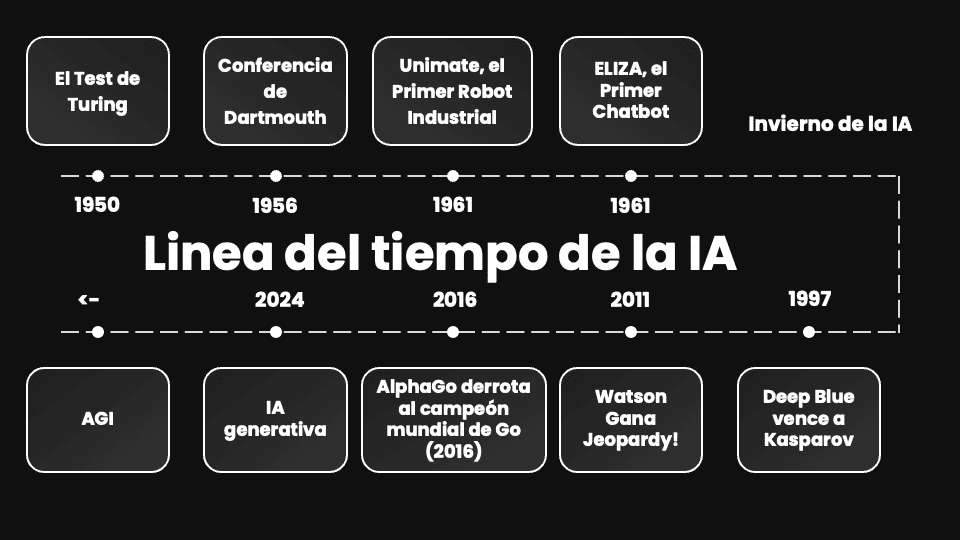
\includegraphics[width=1\linewidth,height=\textheight,keepaspectratio]{modulo1/../img/IAhistoria.png}

}

\caption{\label{fig-historia}\,Principales hitos en la evolución de la
Inteligencia Artificial (1950--2024)}

\end{figure}%

\begin{tcolorbox}[enhanced jigsaw, arc=.35mm, bottomrule=.15mm, bottomtitle=1mm, breakable, colback=white, colbacktitle=quarto-callout-note-color!10!white, colframe=quarto-callout-note-color-frame, coltitle=black, left=2mm, leftrule=.75mm, opacityback=0, opacitybacktitle=0.6, rightrule=.15mm, title=\textcolor{quarto-callout-note-color}{\faInfo}\hspace{0.5em}{Detalle de los hitos históricos (Click para expandir)}, titlerule=0mm, toprule=.15mm, toptitle=1mm]

{\def\LTcaptype{none} % do not increment counter
\begin{longtable}[]{@{}
  >{\raggedright\arraybackslash}p{(\linewidth - 4\tabcolsep) * \real{0.2400}}
  >{\raggedright\arraybackslash}p{(\linewidth - 4\tabcolsep) * \real{0.2400}}
  >{\raggedright\arraybackslash}p{(\linewidth - 4\tabcolsep) * \real{0.5200}}@{}}
\toprule\noalign{}
\begin{minipage}[b]{\linewidth}\raggedright
Año
\end{minipage} & \begin{minipage}[b]{\linewidth}\raggedright
Hito
\end{minipage} & \begin{minipage}[b]{\linewidth}\raggedright
Descripción
\end{minipage} \\
\midrule\noalign{}
\endhead
\bottomrule\noalign{}
\endlastfoot
\textbf{1950} & Test de Turing & Alan\,Turing propuso que una máquina
podía considerarse ``inteligente'' si un ser humano, al conversar con
ella, no podía distinguirla de otra persona. \\
\textbf{1956} & Conferencia\,de\,Dartmouth & Considerada el nacimiento
oficial del término \emph{Inteligencia\,Artificial}. Un grupo de
científicos planteó que las máquinas podrían resolver problemas hasta
entonces exclusivos de los humanos. \\
\textbf{1961} & Unimate & El primer robot industrial. Trabajaba en la
cadena de montaje de General\,Motors, realizando tareas repetitivas y
peligrosas. \\
\textbf{1966} & ELIZA & El primer \emph{chatbot}. Aunque simple y basado
en reglas, demostró el poder del lenguaje natural e hizo creer a muchas
personas que ``tenía sentimientos''. \\
\textbf{1970} & Invierno\,de\,la\,IA & Periodo de frustración
(años\,70\,--\,80) donde las expectativas superaron la tecnología
disponible; los proyectos se estancaron por falta de resultados. \\
\textbf{1997} & Deep\,Blue\,vence\,a\,Kasparov & Un momento histórico
para la humanidad. Por primera vez una computadora derrotó al campeón
mundial de ajedrez, mostrando la capacidad de cálculo de la IA. \\
\textbf{2011} & Watson\,gana\,Jeopardy! & IBM creó una IA capaz de
entender preguntas, bromas y dobles sentidos, para ganar el famoso un
famoso concurso de preguntas en TV. \\
\textbf{2016} & AlphaGo\,derrota\,al\,campeón\,mundial\,de\,Go & El\,Go,
mucho más complejo que el ajedrez, fue conquistado por la
IA\,de\,Google\,DeepMind, que usó estrategias nunca vistas por
humanos. \\
\textbf{2024} & IA Generativa & La\,era\,actual: La IA ha evolucionado:
ya no solo simula el análisis de datos existentes, sino que ahora simula
la capacidad creativa para generar imágenes, música y textos desde
cero. \\
\end{longtable}
}

\end{tcolorbox}

\section{¿Sabías que\ldots?
(Curiosidades)}\label{sabuxedas-que-curiosidades}

\begin{itemize}
\tightlist
\item
  \textbf{Ajedrez:} En 1997, IBM demostró que la fuerza bruta de cálculo
  podía vencer a la intuición humana.
\item
  \textbf{El término:} La palabra ``Inteligencia Artificial'' fue
  acuñado en 1956 por John McCarthy durante la Conferencia de Dartmouth,
  marcando el inicio formal del campo de estudio.
\end{itemize}

\begin{quote}
``La IA ya no se limita a \textbf{simular el análisis} de la
información; hoy, \textbf{simula la creación} misma, generando contenido
original (textos, arte, código) que antes era terreno exclusivo del ser
humano.''
\end{quote}

\subsection{\texorpdfstring{\textbf{El\,futuro\,--\,AGI\,(Inteligencia\,Artificial\,General)}}{El\,futuro\,--\,AGI\,(Inteligencia\,Artificial\,General)}}\label{el-futuro-agi-inteligencia-artificial-general}

El\,gran\,objetivo:
una\,IA\,capaz\,de\,aprender\,y\,realizar\,cualquier\,tarea\,intelectual\,humana\,de\,forma\,autónoma.
Aunque aún estamos lejos de lograrlo, el avance hacia la AGI plantea
preguntas profundas sobre la naturaleza de la inteligencia y el papel de
los humanos en un mundo cada vez más automatizado.

\begin{tcolorbox}[enhanced jigsaw, arc=.35mm, bottomrule=.15mm, bottomtitle=1mm, breakable, colback=white, colbacktitle=quarto-callout-important-color!10!white, colframe=quarto-callout-important-color-frame, coltitle=black, left=2mm, leftrule=.75mm, opacityback=0, opacitybacktitle=0.6, rightrule=.15mm, title=\textcolor{quarto-callout-important-color}{\faExclamation}\hspace{0.5em}{🧠 Gran Debate: ¿La IA piensa o solo calcula?}, titlerule=0mm, toprule=.15mm, toptitle=1mm]

``Si la IA ya simula la creación tan bien que nos cuesta distinguirla,
¿la línea que nos separa de las máquinas está en lo que hacemos o en
cómo lo hacemos?''

\end{tcolorbox}

\section{Dinámica de clase: El Oráculo de la
IA}\label{dinuxe1mica-de-clase-el-oruxe1culo-de-la-ia}

\emph{¿Qué creéis que la IA NUNCA podrá sustituir en vuestro trabajo
diario?} (Anotar las respuestas en la pizarra para debatirlas al final
de la jornada).

\begin{quote}
``La IA ya no se limita a \textbf{simular el análisis} de la
información; hoy, \textbf{simula la creación} misma, generando contenido
original (textos, arte, código) que antes era terreno exclusivo del ser
humano.''
\end{quote}

\subsection{¿Qué significa esto en el día a
día?}\label{quuxe9-significa-esto-en-el-duxeda-a-duxeda}

\begin{itemize}
\tightlist
\item
  \textbf{Antes:} La IA nos decía si un correo era Spam.
\item
  \textbf{Ahora:} La IA escribe el correo por nosotros, imitando nuestro
  estilo.
\end{itemize}

\textbf{Pregunta para la clase:} Si una máquina puede simular
perfectamente tu trabajo creativo\ldots{} ¿cuál es tu nuevo valor
añadido como profesional?

\begin{tcolorbox}[enhanced jigsaw, arc=.35mm, bottomrule=.15mm, bottomtitle=1mm, breakable, colback=white, colbacktitle=quarto-callout-important-color!10!white, colframe=quarto-callout-important-color-frame, coltitle=black, left=2mm, leftrule=.75mm, opacityback=0, opacitybacktitle=0.6, rightrule=.15mm, title=\textcolor{quarto-callout-important-color}{\faExclamation}\hspace{0.5em}{🧠 Gran Debate: ¿La IA piensa o solo calcula?}, titlerule=0mm, toprule=.15mm, toptitle=1mm]

Muchos dicen que la IA ya ``piensa''. Otros, que es solo una simulación
matemática extremadamente avanzada.

\textbf{¿Qué creen ustedes?} ¿Puede una máquina realmente ``entender'' o
solo imita patrones?

\end{tcolorbox}

\section{1.1. La IA como Herramienta de
Predicción}\label{la-ia-como-herramienta-de-predicciuxf3n}

La IA se basa en algoritmos que analizan grandes cantidades de datos
para identificar patrones y hacer predicciones. Esto es fundamental para
aplicaciones como la predicción del clima, recomendaciones de productos
y detección de fraudes.

\begin{figure}

\begin{minipage}[t]{0.50\linewidth}

\begin{figure}[H]

{\centering \pandocbounded{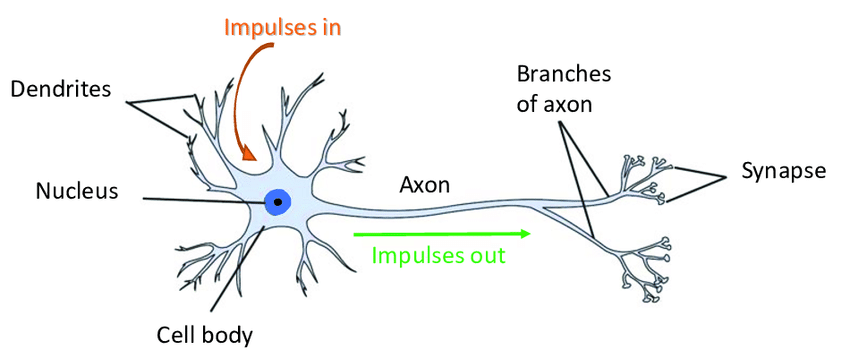
\includegraphics[keepaspectratio]{modulo1/../img/neurona_bio.png}}

}

\subcaption{Neurona Biológica}

\end{figure}%

\end{minipage}%
%
\begin{minipage}[t]{0.50\linewidth}

\begin{figure}[H]

{\centering \pandocbounded{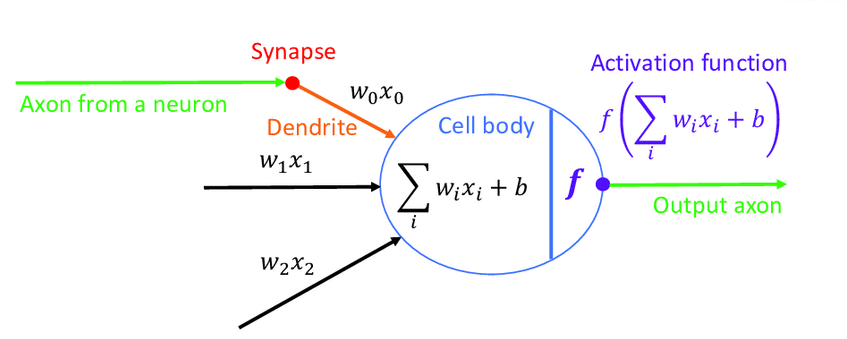
\includegraphics[keepaspectratio]{modulo1/../img/neurona_art.png}}

}

\subcaption{Neurona Artificial}

\end{figure}%

\end{minipage}%

\end{figure}%

\begin{itemize}
\tightlist
\item
  \textbf{Ejemplo:} Predicción del clima, recomendaciones de productos,
  detección de fraudes.
\end{itemize}

\section{2. La IA como Herramienta de Predicción}\label{sec-prediccion}

{[}cite\_start{]}La Inteligencia Artificial moderna no opera mediante
reglas rígidas, sino que se basa en algoritmos que analizan grandes
volúmenes de datos para identificar patrones y generar
\textbf{predicciones} probabilísticas{[}cite: 26{]}.
{[}cite\_start{]}Este enfoque es el que permite aplicaciones críticas
como la detección de fraudes, recomendaciones personalizadas o la
predicción climática{[}cite: 27, 28{]}.

\subsection{El Modelo Fundacional: La Neurona
Artificial}\label{el-modelo-fundacional-la-neurona-artificial}

{[}cite\_start{]}Para comprender cómo predice una máquina, debemos
observar su unidad básica de cálculo, la cual imita el comportamiento de
las neuronas biológicas{[}cite: 32{]}.

\begin{figure*}

\centering{

\pandocbounded{\includegraphics[keepaspectratio]{modulo1/../img/comparativa_neuronas.png}}

}

\caption{\label{fig-neuronas}Comparación entre la estructura de una
neurona biológica y el modelo matemático de un perceptrón (neurona
artificial).}

\end{figure*}%

\subsubsection{¿Cómo funciona este
proceso?}\label{cuxf3mo-funciona-este-proceso}

{[}cite\_start{]}Una neurona artificial es una unidad de cálculo que
procesa información siguiendo estos pasos lógicos{[}cite: 32{]}:

\begin{enumerate}
\def\labelenumi{\arabic{enumi}.}
\tightlist
\item
  {[}cite\_start{]}\textbf{Entradas (\(x\)):} Recibe un vector de datos
  provenientes del exterior o de otras neuronas{[}cite: 32{]}.
\item
  {[}cite\_start{]}\textbf{Pesos (\(w\)):} Cada entrada tiene un peso
  asociado que indica su importancia relativa en el proceso de
  decisión{[}cite: 32{]}.
\item
  {[}cite\_start{]}\textbf{Regla de Propagación:} El sistema multiplica
  cada entrada por su peso, suma todos los resultados y añade un
  \textbf{sesgo (\(b\))} para ajustar la sensibilidad del modelo{[}cite:
  32{]}.
\item
  {[}cite\_start{]}\textbf{Función de Activación (\(f\)):} El resultado
  final se pasa por una función que decide si la neurona se ``excita''
  (genera una salida activa) o permanece inactiva{[}cite: 32{]}.
  {[}cite\_start{]}Este resultado final es lo que conocemos como
  \textbf{activación}{[}cite: 32{]}.
\end{enumerate}

\begin{tcolorbox}[enhanced jigsaw, arc=.35mm, bottomrule=.15mm, bottomtitle=1mm, breakable, colback=white, colbacktitle=quarto-callout-important-color!10!white, colframe=quarto-callout-important-color-frame, coltitle=black, left=2mm, leftrule=.75mm, opacityback=0, opacitybacktitle=0.6, rightrule=.15mm, title=\textcolor{quarto-callout-important-color}{\faExclamation}\hspace{0.5em}{Concepto Clave: Aprendizaje vs.~Reglas}, titlerule=0mm, toprule=.15mm, toptitle=1mm]

A diferencia de la programación tradicional, la IA \textbf{aprende de
ejemplos}. {[}cite\_start{]}No se le dictan reglas fijas; el sistema
ajusta automáticamente sus \textbf{pesos (\(w\))} hasta que sus
predicciones coinciden con la realidad{[}cite: 29, 36, 37{]}.

\end{tcolorbox}

\begin{center}\rule{0.5\linewidth}{0.5pt}\end{center}

\subsection{Aplicación Práctica: De las Reglas a la
Predicción}\label{aplicaciuxf3n-pruxe1ctica-de-las-reglas-a-la-predicciuxf3n}

{[}cite\_start{]}Para visualizar este ``salto tecnológico'', comparamos
un sistema de tasación inmobiliaria basado en reglas manuales frente a
uno que utiliza aprendizaje automático{[}cite: 31, 32{]}.

\subsection{💻 Programación Tradicional (Rígida)}

Se basa en sentencias \texttt{if-else}. {[}cite\_start{]}Si el
programador olvida incluir una variable (como ``vistas al mar''), el
sistema es incapaz de valorar esa característica por sí solo{[}cite:
31{]}.

\begin{Shaded}
\begin{Highlighting}[]
\KeywordTok{def}\NormalTok{ tasador\_manual(metros, zona):}
\NormalTok{    precio\_base }\OperatorTok{=}\NormalTok{ metros }\OperatorTok{*} \DecValTok{1500}
    \ControlFlowTok{if}\NormalTok{ zona }\OperatorTok{==} \StringTok{"Centro"}\NormalTok{:}
        \ControlFlowTok{return}\NormalTok{ precio\_base }\OperatorTok{+} \DecValTok{50000}
    \ControlFlowTok{elif}\NormalTok{ zona }\OperatorTok{==} \StringTok{"Playa"}\NormalTok{:}
        \ControlFlowTok{return}\NormalTok{ precio\_base }\OperatorTok{+} \DecValTok{80000}
    \ControlFlowTok{else}\NormalTok{:}
        \ControlFlowTok{return}\NormalTok{ precio\_base}

\BuiltInTok{print}\NormalTok{(}\SpecialStringTok{f"Precio (Reglas): }\SpecialCharTok{\{}\NormalTok{tasador\_manual(}\DecValTok{80}\NormalTok{, }\StringTok{\textquotesingle{}Centro\textquotesingle{}}\NormalTok{)}\SpecialCharTok{\}}\SpecialStringTok{€"}\NormalTok{)}
\end{Highlighting}
\end{Shaded}

\begin{verbatim}
Precio (Reglas): 170000€
\end{verbatim}

💡 \textbf{Nota:} La IA aprende de ejemplos, no de reglas fijas.

\ldots.. \#\# 3. Algoritmos Tradicionales vs.~Modelos de Aprendizaje ⚙️
\#\#\# 💻 Recurso Interactivo: El Salto Tecnológico

Observad la diferencia entre dar una orden rígida y dejar que el sistema
aprenda.

\subsubsection{1. Programación Tradicional (Reglas
fijas)}\label{programaciuxf3n-tradicional-reglas-fijas}

En este modelo, si el programador olvida una regla (ej. ``vistas al
mar''), el precio nunca cambiará aunque la casa sea preciosa.

\subsection{Recurso Interactivo: El Salto
Tecnológico}\label{recurso-interactivo-el-salto-tecnoluxf3gico}

Aquí compararemos un sistema basado en reglas (If-Else) frente a uno
predictivo.

🛠️ Recurso Práctico: De las Reglas a la Predicción Para experimentar con
estos conceptos, utilizaremos Google Colab, una herramienta que te
permite ejecutar código en la nube sin instalar nada en tu ordenador.

\begin{Shaded}
\begin{Highlighting}[]
\CommentTok{\# Ejemplo de programación tradicional}
\KeywordTok{def}\NormalTok{ tasador\_manual(metros, zona):}
\NormalTok{    precio\_base }\OperatorTok{=}\NormalTok{ metros }\OperatorTok{*} \DecValTok{1500}
    
    \CommentTok{\# Aquí definimos las "reglas"}
    \ControlFlowTok{if}\NormalTok{ zona }\OperatorTok{==} \StringTok{"Centro"}\NormalTok{:}
        \ControlFlowTok{return}\NormalTok{ precio\_base }\OperatorTok{+} \DecValTok{50000}
    \ControlFlowTok{elif}\NormalTok{ zona }\OperatorTok{==} \StringTok{"Playa"}\NormalTok{:}
        \ControlFlowTok{return}\NormalTok{ precio\_base }\OperatorTok{+} \DecValTok{80000}
    \ControlFlowTok{else}\NormalTok{:}
        \ControlFlowTok{return}\NormalTok{ precio\_base}

\CommentTok{\# Prueba cambiando los valores abajo:}
\NormalTok{resultado }\OperatorTok{=}\NormalTok{ tasador\_manual(}\DecValTok{80}\NormalTok{, }\StringTok{"Centro"}\NormalTok{)}
\BuiltInTok{print}\NormalTok{(}\SpecialStringTok{f"Precio calculado por reglas: }\SpecialCharTok{\{}\NormalTok{resultado}\SpecialCharTok{\}}\SpecialStringTok{€"}\NormalTok{)}
\end{Highlighting}
\end{Shaded}

\begin{verbatim}
Precio calculado por reglas: 170000€
\end{verbatim}

En este ejemplo, el modelo de aprendizaje puede ajustar su predicción
basándose en los datos, mientras que la programación tradicional no
puede adaptarse a nuevas situaciones sin modificar el código.

\begin{enumerate}
\def\labelenumi{\arabic{enumi}.}
\setcounter{enumi}{1}
\tightlist
\item
  El modelo de ``IA'' (Aprendizaje Automático) 🧠 Ahora, en lugar de
  escribir reglas, vamos a darle ejemplos a la IA para que ella
  ``deduzca'' cuánto vale cada característica. Verás que no es magia,
  sino un ajuste matemático de pesos.
\end{enumerate}

\begin{Shaded}
\begin{Highlighting}[]
\ImportTok{import}\NormalTok{ numpy }\ImportTok{as}\NormalTok{ np}
\ImportTok{from}\NormalTok{ sklearn.linear\_model }\ImportTok{import}\NormalTok{ LinearRegression}
\CommentTok{\# Datos de ejemplo: metros cuadrados, zona (0=Interior, 1=Playa), precio}
\NormalTok{X }\OperatorTok{=}\NormalTok{ np.array([[}\DecValTok{80}\NormalTok{, }\DecValTok{0}\NormalTok{], [}\DecValTok{80}\NormalTok{, }\DecValTok{1}\NormalTok{], [}\DecValTok{100}\NormalTok{, }\DecValTok{0}\NormalTok{], [}\DecValTok{100}\NormalTok{, }\DecValTok{1}\NormalTok{], [}\DecValTok{120}\NormalTok{, }\DecValTok{0}\NormalTok{], [}\DecValTok{120}\NormalTok{, }\DecValTok{1}\NormalTok{]])}
\NormalTok{y }\OperatorTok{=}\NormalTok{ np.array([}\DecValTok{120000}\NormalTok{, }\DecValTok{200000}\NormalTok{, }\DecValTok{150000}\NormalTok{, }\DecValTok{250000}\NormalTok{, }\DecValTok{180000}\NormalTok{, }\DecValTok{300000}\NormalTok{])      }
\CommentTok{\# Entrenamos el modelo}
\NormalTok{modelo }\OperatorTok{=}\NormalTok{ LinearRegression() }
\NormalTok{modelo.fit(X, y)}
\CommentTok{\# Prueba con nuevos datos}
\NormalTok{nueva\_casa }\OperatorTok{=}\NormalTok{ np.array([[}\DecValTok{90}\NormalTok{, }\DecValTok{1}\NormalTok{]])  }\CommentTok{\# 90 metros en zona de playa}
\NormalTok{prediccion }\OperatorTok{=}\NormalTok{ modelo.predict(nueva\_casa)}
\BuiltInTok{print}\NormalTok{(}\SpecialStringTok{f"Precio predicho por IA: }\SpecialCharTok{\{}\NormalTok{prediccion[}\DecValTok{0}\NormalTok{]}\SpecialCharTok{:.2f\}}\SpecialStringTok{€"}\NormalTok{)}
\end{Highlighting}
\end{Shaded}

\begin{verbatim}
Precio predicho por IA: 230000.00€
\end{verbatim}

\section{4. IA de Película vs.~IA de
Bolsillo}\label{ia-de-peluxedcula-vs.-ia-de-bolsillo}

\begin{itemize}
\tightlist
\item
  \textbf{IA General (Ficción):} El mito de Terminator.
\item
  \textbf{IA Estrecha (Realidad):} Netflix, Google Maps y ChatGPT.
\end{itemize}

\section{5. Cierre: Tu primer Prompt
efectivo}\label{cierre-tu-primer-prompt-efectivo}

Para que la IA pase de darnos respuestas genéricas a soluciones
brillantes, usaremos la fórmula \textbf{R-T-C}:

\begin{enumerate}
\def\labelenumi{\arabic{enumi}.}
\tightlist
\item
  \textbf{R}ol: Dile quién debe ser (ej: ``Actúa como un experto
  en\ldots{}'')
\item
  \textbf{T}area: Qué quieres que haga exactamente (ej: ``Escribe un
  resumen de\ldots{}'')
\item
  \textbf{C}ontexto: Detalles que limitan o guían (ej: ``Para un público
  principiante y en menos de 100 palabras'').
\end{enumerate}

\subsection{🚀 ¡Pruébalo ahora!}\label{pruuxe9balo-ahora}

Copia y completa este ejemplo en ChatGPT: \textgreater{} \emph{``Actúa
como un \textbf{{[}Rol: Profesor de secundaria{]}}. Explica
\textbf{{[}Tarea: qué es una neurona artificial{]}} usando una analogía
sobre \textbf{{[}Contexto: el funcionamiento de una fábrica{]}}.''}

\section{6. Evaluación ✍️}\label{evaluaciuxf3n}

\subsection{Ejercicio práctico: Crea tu propio
Prompt}\label{ejercicio-pruxe1ctico-crea-tu-propio-prompt}

\section{7. Entraga de la solución}\label{entraga-de-la-soluciuxf3n}

\subsection{A través de Moodle: Subir un documento con el prompt que has
creado y la respuesta que te ha dado la
IA.}\label{a-travuxe9s-de-moodle-subir-un-documento-con-el-prompt-que-has-creado-y-la-respuesta-que-te-ha-dado-la-ia.}

\chapter{2. Diferenciando Tipos de Inteligencia
Artificial}\label{diferenciando-tipos-de-inteligencia-artificial}

\section{IA Débil}\label{ia-duxe9bil}

La IA débil, también denominada IA estrecha, es la forma más común y
extendida de IA. Está diseñada para realizar tareas específicas con
precisión y eficiencia, sin comprender realmente lo que hace. Desde
asistentes de voz hasta algoritmos de recomendación, esta tecnología ya
está presente en casi todos los aspectos de nuestra vida cotidiana.

A diferencia de la IA General (AGI), que busca igualar la inteligencia
humana en múltiples ámbitos, la IA Débil se enfoca en una tarea
concreta. No tiene consciencia ni capacidad de aprendizaje más allá de
los datos que le han suministrado.

\textbf{Ejemplos en tu día a día:}

\begin{itemize}
\tightlist
\item
  \textbf{Filtros de Spam:} Solo deciden si un mail es basura.
\item
  \textbf{Reconocimiento facial:} Solo compara puntos de tu cara para
  desbloquear el móvil.
\item
  \textbf{ChatGPT:} Aunque parece que sabe de todo, su ``tarea única''
  es la predicción lingüística.
\end{itemize}

Esta tecnología se basa en modelos de Machine Learning y Deep Learning,
que permiten mejorar su precisión con el tiempo, pero sin alcanzar una
verdadera autonomía.

\section{Aplicaciones de la Inteligencia Artificial
Débil}\label{aplicaciones-de-la-inteligencia-artificial-duxe9bil}

La IA débil es la más utilizada porque lleva años integrándose en
nuestras vidas. Aunque sus aplicaciones son archiconocidas, es vital
recordar cómo impactan en cada sector:

\subsection{🏢 Automatización y
Empresa}\label{automatizaciuxf3n-y-empresa}

El uso de \textbf{Chatbots inteligentes} para atención al cliente y
herramientas de análisis que procesan grandes volúmenes de datos para
optimizar decisiones de negocio.

\subsection{📱 Asistentes Virtuales}\label{asistentes-virtuales}

Sistemas como \textbf{Siri o Google Assistant} que procesan comandos de
voz para facilitar tareas diarias, mejorando continuamente gracias al
aprendizaje profundo.

\subsection{💰 Finanzas y algoritmos}\label{finanzas-y-algoritmos}

\begin{itemize}
\tightlist
\item
  \textbf{Detección de fraude:} Bancos que analizan patrones sospechosos
  en segundos.
\item
  \textbf{Recomendación:} El algoritmo de \textbf{TikTok, Spotify o
  Amazon} que personaliza lo que ves para mejorar tu experiencia.
\end{itemize}

\subsection{🏥 Medicina y Salud}\label{medicina-y-salud}

La ANI permite diagnósticos más rápidos. Los algoritmos de imagen médica
ayudan a detectar enfermedades como el cáncer en etapas muy tempranas,
salvando vidas gracias a su precisión.

``La IA débil no intenta ser un humano; intenta ser la mejor herramienta
posible para una tarea específica.''

El Motor de la IA Débil: Machine Learning Gran parte del éxito de la IA
Débil (ANI) no reside en una programación rígida, sino en su capacidad
para extraer conocimiento de los datos. No es magia, sino matemáticas
aplicadas a través de tres enfoques fundamentales que definen cómo
``aprende'' un algoritmo:

\begin{enumerate}
\def\labelenumi{\arabic{enumi}.}
\tightlist
\item
  Aprendizaje Supervisado
\end{enumerate}

\begin{itemize}
\tightlist
\item
  Es el método más común, donde el sistema aprende a partir de un
  conjunto de datos etiquetados. El ser humano actúa como un guía,
  proporcionando la respuesta correcta (entrada y salida) para que el
  modelo aprenda a predecir resultados futuros.
\end{itemize}

\textbf{Contexto:} Se utiliza principalmente para tareas de
clasificación y regresión.

Caso típico: La detección de spam en el correo electrónico, donde
entrenamos al sistema con millones de ejemplos de mensajes basura frente
a mensajes legítimos.

\begin{enumerate}
\def\labelenumi{\arabic{enumi}.}
\setcounter{enumi}{1}
\tightlist
\item
  Aprendizaje No Supervisado
\end{enumerate}

\begin{itemize}
\tightlist
\item
  En este enfoque, la máquina se enfrenta a los datos sin etiquetas ni
  instrucciones previas. Su objetivo es descubrir estructuras, patrones
  o agrupaciones ocultas de forma autónoma.
\end{itemize}

\textbf{Contexto:}: Ideal para el descubrimiento de patrones que el ojo
humano no detecta a simple vista.

Caso típico: La segmentación de clientes en marketing, donde la IA
agrupa perfiles con comportamientos de compra similares para
personalizar campañas.

\begin{enumerate}
\def\labelenumi{\arabic{enumi}.}
\setcounter{enumi}{2}
\tightlist
\item
  Aprendizaje por Refuerzo
\end{enumerate}

\begin{itemize}
\tightlist
\item
  A diferencia de los anteriores, aquí la IA aprende mediante la
  interacción con un entorno. El algoritmo toma decisiones y recibe
  ``premios'' por los aciertos o ``penalizaciones'' por los errores,
  optimizando su comportamiento mediante el ensayo y error.
\end{itemize}

\textbf{Contexto:} Se aplica en entornos dinámicos donde se busca una
estrategia óptima a largo plazo.

Caso típico: La optimización de rutas logísticas en tiempo real o el
entrenamiento de sistemas para juegos de estrategia complejos.

\subsection{📺 Recursos Audiovisuales para
hoy}\label{recursos-audiovisuales-para-hoy}

\begin{itemize}
\tightlist
\item
  \textbf{Simulación visual:}
  \href{https://www.youtube.com/watch?v=HK6y8DAPN_0}{Sora OpenAI}
\item
  \textbf{Simulación de voz/trato:}
  \href{https://www.youtube.com/watch?v=D5VN56jQMWM}{Google Duplex}
\item
  \textbf{Simulación creativa:}
  \href{https://www.youtube.com/watch?v=2_W6S78Xf68}{Música con Suno AI}
\end{itemize}

\subsection{🎵 Experimentación en vivo: Creación con Suno
AI}\label{experimentaciuxf3n-en-vivo-creaciuxf3n-con-suno-ai}

Vamos a poner a prueba la \textbf{IA Generativa} creando una pieza
musical desde cero.

suno.com

\begin{itemize}
\tightlist
\item
  \textbf{Paso 1:} Elegimos un tema común de la clase.
\item
  \textbf{Paso 2:} Definimos el estilo musical (¿Flamenco? ¿Heavy Metal?
  ¿Trap?).
\item
  \textbf{Paso 3:} Observamos cómo la IA \textbf{simula} la composición,
  la voz y la instrumentación.
\end{itemize}

\textbf{Reflexión post-audición:} ¿Podríais distinguir esta canción de
una real en la radio? Si la respuesta es ``no'', ¿cambia vuestra
definición de ``creatividad''?

La versión gratuita tiene créditos limitados.

Privacidad: Recuérdales (esto queda muy bien como profesor) que al usar
estas herramientas ``gratuitas'' a menudo estamos regalando nuestros
datos para entrenar a sus modelos.

\subsection{🧠 La Trampa de la
Creatividad}\label{la-trampa-de-la-creatividad}

Al ver a Suno crear una canción desde cero, es fácil pensar:
\emph{``¡Esto ya es inteligencia real!''}.

Sin embargo, \textbf{Suno sigue siendo IA Débil}. 1. \textbf{No hay
consciencia:} No sabe qué es la tristeza aunque componga un blues
triste; solo replica patrones matemáticos de otros blues. 2. \textbf{Sin
versatilidad:} No puede salir de su función musical. Una IA Fuerte
podría componer la canción y luego explicarte por qué eligió esos
acordes basándose en su propia ``experiencia de vida''.

\section{IA Fuerte (General AI - AGI)}\label{ia-fuerte-general-ai---agi}

Sería una IA capaz de realizar \textbf{cualquier tarea intelectual}
humana.

\begin{itemize}
\tightlist
\item
  \textbf{Multitarea real:} Podría aprender a cocinar, programar y
  escribir poesía por iniciativa propia.
\item
  \textbf{Autonomía:} Tendría objetivos propios, no solo los que le
  programamos.
\item
  \textbf{Estado:} Actualmente es \textbf{ciencia ficción}, aunque
  empresas como OpenAI trabajan para alcanzarla.
\end{itemize}

\section{Comparativa Rápida}\label{comparativa-ruxe1pida}

{\def\LTcaptype{none} % do not increment counter
\begin{longtable}[]{@{}lll@{}}
\toprule\noalign{}
Característica & IA Débil (Hoy) & IA Fuerte (Futuro?) \\
\midrule\noalign{}
\endhead
\bottomrule\noalign{}
\endlastfoot
\textbf{Habilidad} & Especializada & Universal \\
\textbf{Consciencia} & No (Simulación) & Se debate si sería necesaria \\
\textbf{Ejemplo} & Google Maps & Jarvis (Iron Man) \\
\textbf{Propósito} & Resolver tareas & Pensar como humano \\
\end{longtable}
}

\section{Dinámica: ``¿Es IA Débil o
Fuerte?''}\label{dinuxe1mica-es-ia-duxe9bil-o-fuerte}

\emph{Si mañana un robot limpia tu casa perfectamente, pero si le pides
que te ayude con la declaración de la renta te dice que no sabe de qué
hablas\ldots{}}

\textbf{¿Es una IA Débil o Fuerte?} \emph{(Respuesta: Débil, porque está
limitada a su función de limpieza).}

\section{6. Evaluación ✍️}\label{evaluaciuxf3n-1}

\subsection{Ejercicio práctico: Crea tu propio
Prompt}\label{ejercicio-pruxe1ctico-crea-tu-propio-prompt-1}

\section{7. Entraga de la solución}\label{entraga-de-la-soluciuxf3n-1}

\subsection{A través de Moodle: Subir un documento con el prompt que has
creado y la respuesta que te ha dado la
IA.}\label{a-travuxe9s-de-moodle-subir-un-documento-con-el-prompt-que-has-creado-y-la-respuesta-que-te-ha-dado-la-ia.-1}

\chapter{}\label{section-2}

\chapter{4. Procesamiento del lenguaje natural
(NLP)}\label{procesamiento-del-lenguaje-natural-nlp}

\chapter{Untitled}\label{untitled}

\part{Módulo 2 · Desafíos y Avances}

\chapter{}\label{section-3}

\part{Módulo 3 · Aplicaciones Prácticas}

\chapter{}\label{section-4}

\part{Laboratorio y Evaluación}

\chapter{Laboratorio 1: El Problema de Monty
Hall}\label{laboratorio-1-el-problema-de-monty-hall}

Probabilidad, simulación e intuición

\hfill\break

\chapter{¿Podrás vencer a la
probabilidad?}\label{podruxe1s-vencer-a-la-probabilidad}

Este experimento muestra por qué la IA y la estadística se basan en
datos y no en ``corazonadas''.

\begin{tcolorbox}[enhanced jigsaw, arc=.35mm, bottomrule=.15mm, bottomtitle=1mm, breakable, colback=white, colbacktitle=quarto-callout-note-color!10!white, colframe=quarto-callout-note-color-frame, coltitle=black, left=2mm, leftrule=.75mm, opacityback=0, opacitybacktitle=0.6, rightrule=.15mm, title=\textcolor{quarto-callout-note-color}{\faInfo}\hspace{0.5em}{Cómo jugar}, titlerule=0mm, toprule=.15mm, toptitle=1mm]

\begin{enumerate}
\def\labelenumi{\arabic{enumi}.}
\tightlist
\item
  Elige el número de puertas (3 es el caso clásico).
\item
  Elige tu estrategia:

  \begin{itemize}
  \tightlist
  \item
    \textbf{Quedarse} con la primera puerta.
  \item
    \textbf{Cambiar} después de que el presentador abra puertas vacías.
  \end{itemize}
\item
  Pulsa el botón para simular 1.000 partidas.
\end{enumerate}

\end{tcolorbox}

\begin{Shaded}
\begin{Highlighting}[]
\NormalTok{//| panel: sidebar}
\NormalTok{//| label: controles}

\NormalTok{viewof puertas = Inputs.range(}
\NormalTok{  [3, 15],}
\NormalTok{  \{}
\NormalTok{    label: "Número de puertas:",}
\NormalTok{    step: 1,}
\NormalTok{    value: 3}
\NormalTok{  \}}
\NormalTok{)}

\NormalTok{viewof estrategia = Inputs.radio(}
\NormalTok{  ["Quedarse", "Cambiar"],}
\NormalTok{  \{}
\NormalTok{    label: "Estrategia:",}
\NormalTok{    value: "Cambiar"}
\NormalTok{  \}}
\NormalTok{)}

\NormalTok{viewof ejecutar = Inputs.button("Simular 1.000 partidas")}
\end{Highlighting}
\end{Shaded}

\section{Resultados de la
simulación}\label{resultados-de-la-simulaciuxf3n}

\begin{Shaded}
\begin{Highlighting}[]
\NormalTok{//| label: simulacion}

\NormalTok{ejecutar}

\NormalTok{const partidas = 1000}
\NormalTok{let victorias = 0}

\NormalTok{for (let i = 0; i \textless{} partidas; i++) \{}

\NormalTok{  // Puerta con premio}
\NormalTok{  const premio = Math.floor(Math.random() * puertas)}

\NormalTok{  // Primera elección del jugador}
\NormalTok{  const eleccion = Math.floor(Math.random() * puertas)}

\NormalTok{  // Estrategia}
\NormalTok{  if (estrategia === "Quedarse") \{}
\NormalTok{    if (eleccion === premio) victorias++}
\NormalTok{  \} else \{}
\NormalTok{    // Cambiar gana siempre que la elección inicial NO fuera correcta}
\NormalTok{    if (eleccion !== premio) victorias++}
\NormalTok{  \}}
\NormalTok{\}}

\NormalTok{const porcentaje\_simulado = (victorias / partidas) * 100}

\NormalTok{const porcentaje\_teorico =}
\NormalTok{  estrategia === "Quedarse"}
\NormalTok{    ? (1 / puertas) * 100}
\NormalTok{    : ((puertas {-} 1) / puertas) * 100}

\NormalTok{display(\{}
\NormalTok{  simulado: porcentaje\_simulado,}
\NormalTok{  teorico: porcentaje\_teorico}
\NormalTok{\})}
\end{Highlighting}
\end{Shaded}

\begin{Shaded}
\begin{Highlighting}[]
\NormalTok{//| label: grafico}

\NormalTok{Plot.plot(\{}
\NormalTok{  title: "Simulación vs Probabilidad Teórica",}
\NormalTok{  width: 700,}
\NormalTok{  height: 450,}

\NormalTok{  marks: [}
\NormalTok{    Plot.barY(}
\NormalTok{      [}
\NormalTok{        \{}
\NormalTok{          tipo: "Simulación",}
\NormalTok{          valor: simulado}
\NormalTok{        \},}
\NormalTok{        \{}
\NormalTok{          tipo: "Teoría",}
\NormalTok{          valor: teorico}
\NormalTok{        \}}
\NormalTok{      ],}
\NormalTok{      \{}
\NormalTok{        x: "tipo",}
\NormalTok{        y: "valor"}
\NormalTok{      \}}
\NormalTok{    ),}

\NormalTok{    Plot.text(}
\NormalTok{      [}
\NormalTok{        \{}
\NormalTok{          tipo: "Simulación",}
\NormalTok{          valor: simulado}
\NormalTok{        \},}
\NormalTok{        \{}
\NormalTok{          tipo: "Teoría",}
\NormalTok{          valor: teorico}
\NormalTok{        \}}
\NormalTok{      ],}
\NormalTok{      \{}
\NormalTok{        x: "tipo",}
\NormalTok{        y: "valor",}
\NormalTok{        text: d =\textgreater{} \textasciigrave{}$\{d.valor.toFixed(1)\}\%\textasciigrave{},}
\NormalTok{        dy: {-}10}
\NormalTok{      \}}
\NormalTok{    ),}

\NormalTok{    Plot.ruleY([0])}
\NormalTok{  ],}

\NormalTok{  y: \{}
\NormalTok{    domain: [0, 100],}
\NormalTok{    label: "\% de victorias",}
\NormalTok{    grid: true}
\NormalTok{  \}}
\NormalTok{\})}
\end{Highlighting}
\end{Shaded}

\section{¿Qué está ocurriendo?}\label{quuxe9-estuxe1-ocurriendo}

Cuando eliges una puerta al inicio:

\begin{itemize}
\tightlist
\item
  Tu probabilidad inicial de acertar es:
\end{itemize}

\[
\frac{1}{n}
\]

\begin{itemize}
\tightlist
\item
  La probabilidad de que el premio esté en alguna de las otras puertas
  es:
\end{itemize}

\[
\frac{n-1}{n}
\]

Al abrir puertas vacías, esa probabilidad se concentra en la puerta
restante.

\subsection{Caso clásico: 3 puertas}\label{caso-cluxe1sico-3-puertas}

\begin{itemize}
\tightlist
\item
  Quedarse → 33.3\%
\item
  Cambiar → 66.6\%
\end{itemize}

Por eso \textbf{cambiar de puerta duplica la probabilidad de ganar}.

\chapter{}\label{section-5}

\chapter{}\label{section-6}

\chapter{}\label{section-7}

\bookmarksetup{startatroot}

\chapter{}\label{section-8}




\end{document}
